\documentclass[12pt]{article}
\usepackage[all, stdclass]{lix}
\usepackage{graphicx}
\usepackage{svg}
\svgsetup{
  inkscapepath=assets/,  % Path to the directory containing your SVG files
  svgpath=assets/        % Path to the directory containing your SVG files
}
\usepackage{float}
\usepackage{hyperref}
\usepackage{times}
\usepackage{amsmath}


%----------EDIT COVER INFO HERE -----------------%

\def \LOGOPATH {assets/birzeit-logo.png}
\def \DEPARTEMENT {Department of Electrical \& Computer Engineering}
\def \COURSENUM {ENEE2103}
\def \COURSENAME {Circuits and Electronics Laboratory}
\def \REPORTTITLE {The Field-Effect Transistor}
\def \STUDENTNAME {Mohammad Abu-Shelbaia}
\def \STUDENTID {1200198}
\def \INSTRUCTOR {Dr. Mahran Quran}
\def \ASSISTANT {Eng. Raffah Rahal}
\def \REPORTNUM {8}

%--------------------BORDERS----------------------------%
% \usepackage{parskip}
% \setlength{\parskip}{0pt}
% \geometry{top=1.54cm}
% \usepackage{everyshi}
% \usepackage{tikz}
% \EveryShipout{%
%     \begin{tikzpicture}[overlay,remember picture]
%         \draw [line width=0.5pt]
%             ($ (current page.north west) + (1cm,-1cm) $)
%             rectangle
%             ($ (current page.south east) + (-1cm,1cm) $);
%     \end{tikzpicture}
% }
%------------------------------------------------%
\begin{document}
\pagenumbering{Roman}

\begin{titlepage}
    \vfill
    \begin{center}
        \includegraphics[width=0.7\textwidth]{\LOGOPATH} \\
        \hfill \\
        \Large{\DEPARTEMENT} \\
        \Large{\COURSENUM\;-\;\COURSENAME} \\
        \vfill
        \textbf{\LARGE{Experiment \#\REPORTNUM}} \\
        \textbf{\LARGE{\REPORTTITLE}}
    \end{center}
    \vfill
    \begin{flushleft}
        \Large{\textbf{Prepared by:}\\ \STUDENTNAME\quad\STUDENTID} \\

        \Large{\textbf{Instructor:} \INSTRUCTOR} \\
        \Large{\textbf{Assistant:} \ASSISTANT} \\
        \Large{\textbf{Section:} 4}\\
        \LARGE{\textbf{ }}\\
        \LARGE{\textbf{ }}\\
        \LARGE{\textbf{ }}\\
        \Large{\textbf{Date:} \today}\\
    \end{flushleft}
    \vfill
\end{titlepage}


%--------------- TABLES --------------------------------%
\tableofcontents
\clearpage
\setlength{\parskip}{\baselineskip}%
\listoffigures
\clearpage

\pagenumbering{arabic}
%-------------- CONTENT ---------------------%
\h{Simulation and Data Analysis}
\hh{Characteristics of the N-JFET}
\begin{figure}[H]
\centering
    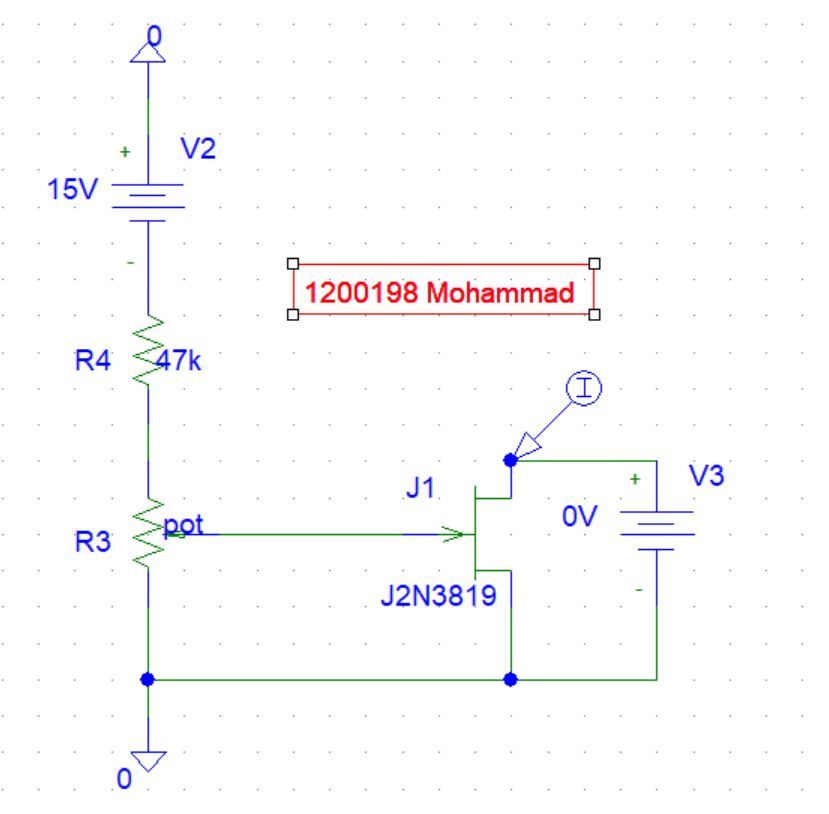
\includegraphics[width=0.5\textwidth]{assets/main/2023-08-18-23-40-04.png}
    \caption{N-CHANNEL JFET Circuit}
\end{figure}
\begin{figure}[H]
    \centering
    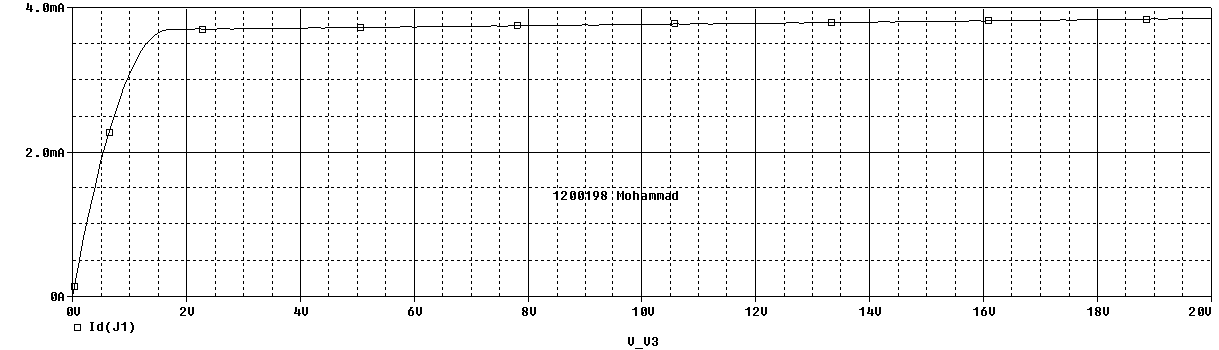
\includegraphics[width=\textwidth]{assets/main/2023-08-18-23-43-53.png}
    \caption{$I_{DS}$ vs. $V_{DS}$}
\end{figure}
From the graph above, Id is unchanged with Vds after it exceeds 2V, Ig is very small and is almost zero.
\hh{Common Drain Amplifier}
\begin{figure}[H]
    \centering
    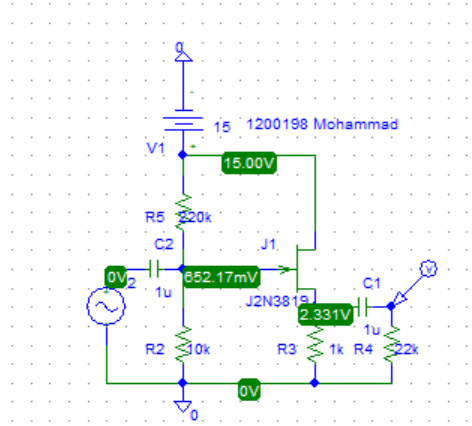
\includegraphics[width=0.5\textwidth]{assets/main/2023-08-18-23-52-56.png}
    \caption{Common Drain Amplifier Circuit}
\end{figure}
From the above circuit, $V_G$ is 652mV and $V_S$ is 2.3V.
\begin{figure}[H]
    \centering
    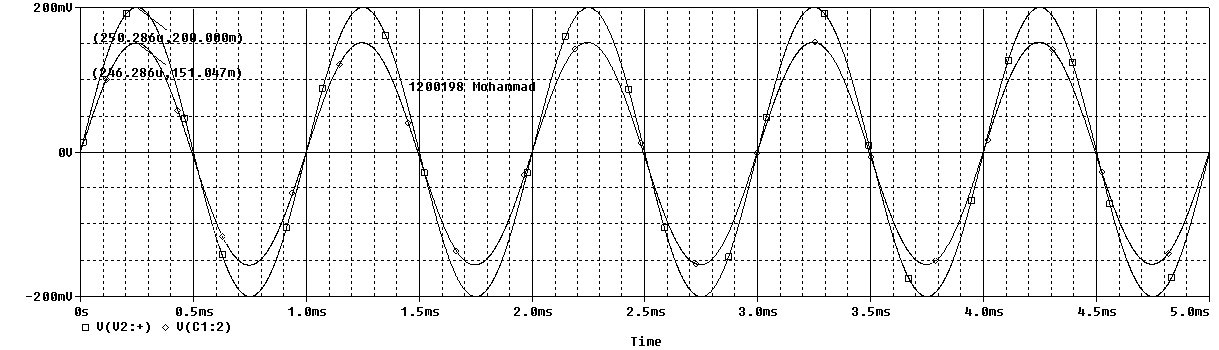
\includegraphics[width=\textwidth]{assets/main/2023-08-19-00-15-23.png}
\end{figure}
from the above graph, the voltage gain is given by:
\begin{equation}
    A_v = \frac{V_{out}}{V_{in}} = \frac{151}{200} = 0.755
\end{equation}
and the phase shift is given by:
\begin{equation}
    \phi = \Delta t \times 360 \times f = {4 \times 360 \times 1000 \over 10^{6}} = 1.44^{\circ}
\end{equation}
\begin{figure}[H]
    \centering
    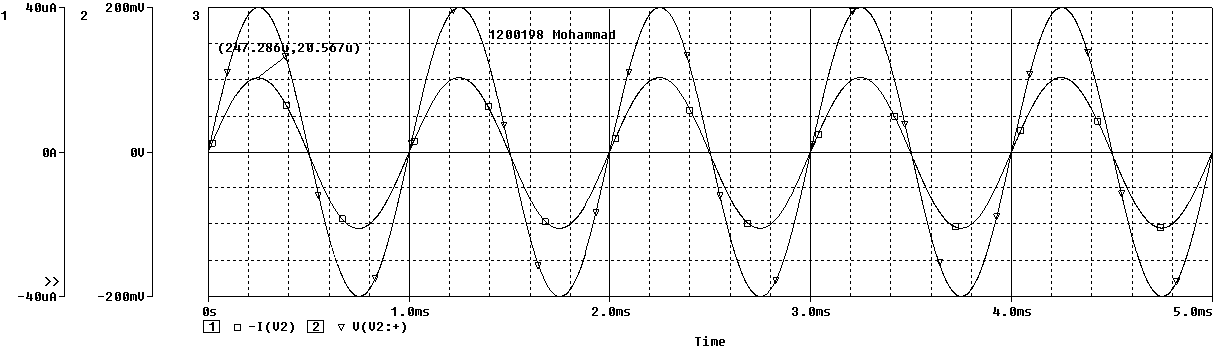
\includegraphics[width=\textwidth]{assets/main/2023-08-19-00-30-43.png}
    \caption{$V_{in}$ and $I_{in}$}
\end{figure}
from the above graph, the input impedance is given by:
\begin{equation}
    Z_{in} = \frac{V_{in}}{I_{in}} = \frac{200\times10^{-3}}{20.567 \time 10^{-6}} = 9.72K\Omega
\end{equation}
\begin{figure}[H]
    \centering
    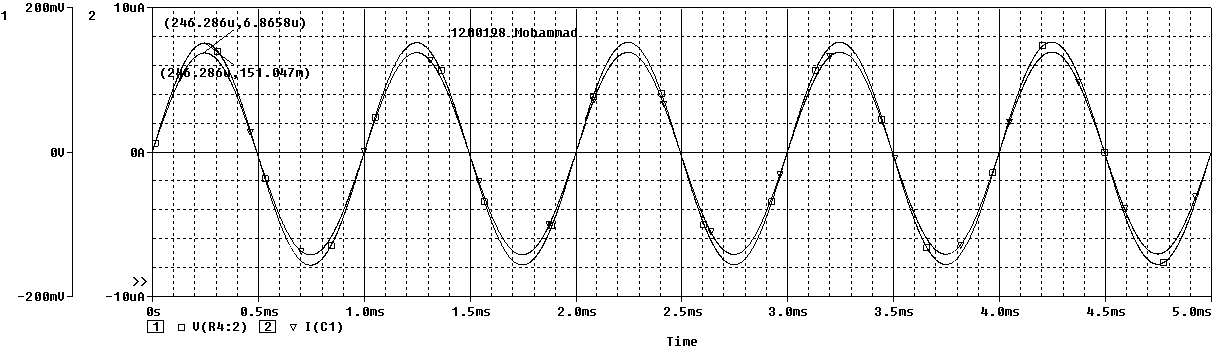
\includegraphics[width=\textwidth]{assets/main/2023-08-19-00-42-46.png}
    \caption{$V_{out}$ and $I_{out}$}
\end{figure}
From the above graph, the output impedance is given by:
\begin{equation}
    Z_{out} = \frac{V_{out}}{I_{out}} = \frac{151.047 \times 10^{-3}}{6.865 \time 10^{-6}} =  22K\Omega     
\end{equation}

\end{document}
